\vspsec
\section{Meta-Learning for Online Model Adaptation}\label{sec:ml4ac}
\vspsec
In this section, we present our approach for meta-learning for online model adaptation. As explained in Section~\ref{sec:prelim-meta}, standard meta-learning formulations require the learned model $\bm{\theta}_*, \bm{\psi}_*$ to learn using $M$ data points from some new ``task.'' In prior gradient-based and model-based meta-RL approaches~\citep{finn2017maml,saemundsson2018meta}, the $M$ has corresponded to $M$ trajectories, leading to episodic adaptation.

Our notion of task is slightly more fluid, where every segment of a trajectory can be considered to be a different ``task,'' and observations from the past $M$ \emph{timesteps} (rather than the past $M$ episodes) can be considered as providing information about the current task setting. 
Since changes in system dynamics, terrain details, or other environmental changes can occur at any time, we consider (at every time step) the problem of adapting the model using the $M$ past time steps to predict the next $K$ timesteps. In this setting, $M$ and $K$  are pre-specified hyperparameters; see appendix for a sensitivity analysis of these parameters.

In this work, we use the notion of environment $\mathcal{E}$ to denote different settings or configurations of a particular problem, ranging from malfunctions in the system's joints to the state of external disturbances. We assume a distribution of environments $\rho({\mathcal{E}})$ that share some common structure, such as the same observation and action space, but may differ in their dynamics $p_\mathcal{E}({\bf s'}|{\bf s}, {\bf a})$. We denote a trajectory segment by $\tau_{\mathcal{E}}(i, j)$, which represents a sequence of states and actions
$({\bf s}_{i}, {\bf a}_{i}, ..., {\bf s}_{j}, {\bf a}_{j}, {\bf s}_{j+1})$ sampled within an environment $\mathcal{E}$. Our algorithm assumes that the environment is locally consistent, in that every segment of length $j-i$ has the same environment. Even though this assumption is not always correct, it allows us to learn to adapt from data without knowing when the environment has changed. Due to the fast nature of our adaptation (less than a second), this assumption is seldom violated.

We pose the meta-RL problem in this setting as an optimization over ($\bm{\theta}$, $\bm{\psi}$) with respect to a maximum likelihood meta-objective. The meta-objective is the likelihood of the data under a predictive model $\hat p_{\bm{\theta}'}({\bf s'}|{\bf s}, {\bf a})$ with parameters $\bm{\theta}'$, where \mbox{$\bm{\theta}' = u_{\bm{\psi}}(\tau_{\mathcal{E}}(t-M, t-1), \bm{\theta})$} corresponds to model parameters that were updated using the past $M$ data points. Concretely, this corresponds to the following optimization:
%
\begin{align}
\label{eq:metaobj}
    \min_{\bm{\theta}, \bm{\psi}} \hspace{4pt} \mathbb{E}_{\tau_{\mathcal{E}}(t-M, t+K) \sim \mathcal{D}}  \big[ \mathcal{L}(\tau_{\mathcal{E}}(t, t+K), \bm{\theta}'_{\mathcal{E}})\big] \hspace{10pt}
\text{s.t.:} \hspace{10pt} \bm{\theta}'_{\mathcal{E}} = u_{\bm{\psi}}(\tau_{\mathcal{E}}(t-M, t-1), \bm{\theta}),
\end{align}
%
In that $\tau_{\mathcal{E}}(t-M, t+K) \sim \mathcal{D}$ corresponds to trajectory segments sampled from our previous experience, and the loss $\mathcal{L}$ corresponds to the negative log likelihood of the data under the model:
%
\begin{align}
\loss(\tau_{\mathcal{E}}(t, t+K), \bm{\theta}_{\mathcal{E}}') \triangleq -\frac{1}{K} 
%\sum_{k = t}^{t+K} 
\sum_{k=t}^{t+K}
\log \hat p_{\bm{\theta}_{\mathcal{E}}'} ( {\bf s}_{k+1} | {\bf s}_{k}, {\bf a}_{k}).
    \label{eq:inner update}
\end{align}
% 
In the meta-objective in Equation~\ref{eq:metaobj}, note that the past $M$ points are used to adapt $\bm{\theta}$ into $\bm{\theta'}$, and the loss of this $\bm{\theta'}$ is evaluated on the future $K$ points. Thus, we use the past $M$ timesteps to provide insight into how to adapt our model to perform well for nearby future timesteps. As outlined in Algorithm~\ref{alg:metatrain}, the update rule $u_{\bm{\psi}}$ for the inner update and a gradient step on $\bm{\theta}$ for the outer update allow us to optimize this meta-objective of adaptation. Thus, we achieve fast adaptation at test time by being able to fine-tune the model using just $M$ data points. 

While we focus on reinforcement learning problems in our experiments, this meta-learning approach could be used for a learning to adapt online in a variety of sequence modeling domains. We present our algorithm using both a recurrence and a gradient-based meta-learner, as we discuss next.

\paragraph{Gradient-Based Adaptive Learner (GrBAL).} GrBAL uses a gradient-based meta-learning to perform online adaptation; in particular, we use MAML~\citep{finn2017maml}. In this case, our update rule is prescribed by gradient descent (~\ref{eq:inner update}.)
%
\begin{align}
\bm{\theta^\prime}_{\mathcal{E}} = u_{\bm{\psi}}(\tau_{\mathcal{E}}(t-M, t-1), \bm{\theta}) = \bm{\theta}_{\mathcal{E}} + \bm{\psi} \nabla_{\bm{\theta}} \frac{1}{M} 
\sum_{m=t-M}^{t-1}
\log \hat p_{\bm{\theta}_{\mathcal{E}}} ( {\bf s}_{m+1} | {\bf s}_{m}, {\bf a}_{m})
    \label{eq:inner update}
\vspace{-0.2in}
\end{align}
%
\paragraph{Recurrence-Based Adaptive Learner (ReBAL).} ReBAL, instead, utilizes a recurrent model, which  learns its own update rule (i.e., through its internal gating structure). In this case, $\bm\psi$ and $u_{\bm\psi}$ correspond to the weights of the recurrent model that update its hidden state.
% 
\begin{figure*}
\noindent
\begin{minipage}[t]{0.5\textwidth}
\begin{algorithm}[H]
\begin{algorithmic}[1]
 \REQUIRE Distribution $\rho_{\mathcal{E}}$ over tasks
 \REQUIRE Learning rate $\beta \in \mathbb{R}^+$
 \REQUIRE Number of sampled tasks $N$, dataset $\mathcal{D}$
 \REQUIRE Task sampling frequency $n_{S} \in \mathbb{Z}^{+}$
 \STATE Randomly initialize $\bm{\theta}$
\FOR{$i = 1, ...$}
\IF{$i \bmod n_S = 0$}
\STATE Sample $\mathcal{E} \sim \rho(\mathcal{E})$
\STATE Collect $\tau_{\mathcal{E}}$ using Alg.~\ref{alg:generic}
\STATE $\mathcal{D} \leftarrow \mathcal{D} \cup \{\tau_{\mathcal{E}}\}$
\ENDIF
    \FOR{$j=1 \dots N$}
    \STATE $\tau_{\mathcal{E}}(t-M, t-1), \tau_{\mathcal{E}}(t, t+K) \sim \mathcal{D}$
    \STATE $\bm{\theta}'_{\mathcal{E}} \leftarrow u_{\bm{\psi}}(\tau_{\mathcal{E}}(t-M, t-1), \bm{\theta})$
    \STATE $\mathcal{L}_j  \leftarrow \mathcal{L} (\tau_{\mathcal{E}}(t, t+K), {\bm{\theta}'_{\mathcal{E}}})$
    \ENDFOR
    \STATE $\bm{\theta} \leftarrow \bm{\theta} - \beta \nabla_{\bm{\theta}} \frac{1}{N} \sum\limits_{j=1}^N \mathcal{L}_j$
    \STATE $\bm{\psi} \leftarrow \bm{\psi} - \eta \nabla_{\bm{\psi}}  \frac{1}{N} \sum\limits_{j=1}^N \mathcal{L}_j$
\ENDFOR
\STATE Return (${\bm{\theta}}$, $\bm{\psi}$) as (${\bm{\theta}_*}$, $\bm{\psi_*}$)
\end{algorithmic}
\caption{Model-Based Meta-Reinforcement Learning (train time)}
\label{alg:metatrain}
\end{algorithm}
\end{minipage}
\noindent
\hspace{0.1cm}
\begin{minipage}[t]{0.45\textwidth}
\noindent
\begin{algorithm}[H]
\begin{algorithmic}[1]
 \REQUIRE Meta-learned parameters $\bm{\theta}_*, \bm{\psi}_*$
 \REQUIRE controller$()$, $H$, $r$, $n_{A}$
\STATE $\data \leftarrow \emptyset $\\
\FOR{ \text{each timestep $t$}}
    \STATE $\bm{\theta}_*' \leftarrow u_{\bm{\psi_*}}(\data(t-M, t-1), \bm{\theta}_*)$\\
    \STATE ${\bf a }\leftarrow$ controller$({\bm{\theta}_*'},r,H,n_{A})$\\
    \STATE Execute ${\bf a}$, add result to $\data$
\ENDFOR
\STATE Return rollout $\data$
\end{algorithmic}
\caption{Online Model Adaptation\\(test time)}
\label{alg:generic}
\end{algorithm}
\centering
\vspace{-0.3cm}

\includegraphics[width=.42\textwidth]{pictures/envs/crippled_cheetah.png}
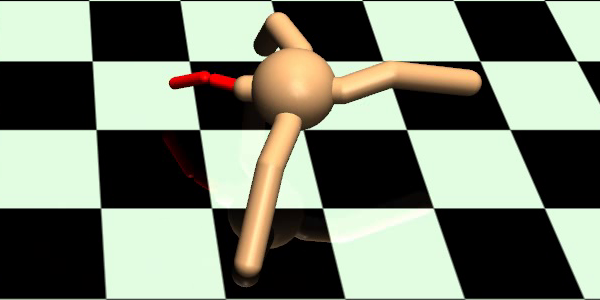
\includegraphics[width=.42\textwidth]{pictures/envs/mujoco_ant.png}\\

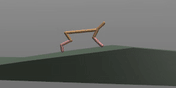
\includegraphics[width=.42\textwidth]{pictures/envs/mujoco_hfield.png}

\includegraphics[width=.42\textwidth]{pictures/envs/mujoco_pier.png}\\
\hspace{0.02cm}

\includegraphics[width=.42\textwidth]{pictures/roach_adapt/roach_slope.jpg}

\includegraphics[width=.42\textwidth]{pictures/roach_adapt/roach_leg_crop.jpg}
\vspace{-0.2cm}
\caption[width=0.4\textwidth]{\small Two real-world and four simulated environments on which our method is evaluated and adaptation is crucial for success (e.g., adapting to different slopes and leg failures)}
%\TODO{Add picture of the roach}.}
\vspace{-0.1cm}
\label{fig:mujoco-envs}
\end{minipage}
\vspace{-0.2 in}
\end{figure*}


\vspsec
\section{Model-Based Meta-Reinforcement Learning}\label{sec:generic_alg}
\vspsec
Now that we have discussed our approach for enabling online adaptation, we next propose how to build upon this idea to develop a model-based meta-reinforcement learning algorithm.
First, we explain how the agent can use the adapted model to perform a task, given parameters $\bm{\theta}_*$ and $ \bm{\psi}_*$ from optimizing the meta-learning objective.

Given  $\bm{\theta}_*$ and $ \bm{\psi}_*$, we use the agent's recent experience to adapt the model parameters: $\bm{\theta}_*^\prime = u_{\bm{\psi}_*}(\tau(t-M, t), \bm{\theta}_*)$. This results in a model $\hat{p}_{\bm{\theta_*^\prime}}$ that better captures the local dynamics in the current setting, task, or environment. This adapted model is then passed to our controller, along with the reward function $r$ and a planning horizon $H$. We use a planning $H$ that is smaller than the adaptation horizon $K$, since the adapted model is only valid within the current context. We use model predictive path integral control (MPPI)~\citep{williams15mppi}, but, in principle, our model adaptation approach is agnostic to the model predictive control (MPC) method used.

The use of MPC compensates for model inaccuracies by preventing accumulating errors, since we replan at each time step using updated state information. MPC also allows for further benefits in this setting of online adaptation, because the model $\hat p_{\bm{\theta}_\mathcal{E}'}$ itself will also improve by the next time step. After taking each step, we append the resulting state transition onto our dataset, reset the model parameters back to $\bm{\theta}_*$, and repeat the entire planning process for each timestep. See Algorithm~\ref{alg:generic} for this adaptation procedure. Finally, in addition to test-time, we also perform this online adaptation procedure during the meta-training phase itself, to provide on-policy rollouts for meta-training. For the complete meta-RL algorithm, see  Algorithm~\ref{alg:metatrain}.
